\section{Auswertung}
\label{sec:Auswertung}
Für die Auswertung werden die folgende Größen benötigt.
\begin{align*}
  \text{Volumen der Behälter: } V &= 3.0 \,\si{\liter} \\
  \text{spezifische Wärmekapazität}\, c_\symup{p} &= 75.38\si{\frac{\joule}{\mol\,\kelvin}}  \\
  \text{Dichte Wasser } \rho_\symup{Wasser} &= 55.39 \,\si{\frac{\mol}{\liter}}
        (\text{bei } 294.85 \si{\kelvin} \text{ und } 1\si{\bar}) \\
  \text{molare Masse von } \ce{Cl2F2C}: M &= 120.91 \si{\frac{\gram}{\mol}} \\
  p_0 &= 1.0 \si{\frac{\kilo\gram}{\meter^2}}  \\
  \rho_0 &= 5.51  \si{\frac{\kilo\gram}{\meter^3}} \\
  T_0 &= 273.15 \,  \si{\kelvin}  \\
  m_2c_\symup{w} &= 12525.67 \si{\frac{\joule}{\kelvin}} \\
  m_\symup{k}c_\symup{k} &= 660   \si{\frac{\joule}{\kelvin}}
\end{align*}
Die Werte zur Wasser Dichte und zur spezifischen Wärmekapazität stammen von
http://www.nist.gov/ (15.11.2015) und molare Masse von http://de.webqc.org/molecular-weight-of-Cl2F2C.html (15.11.2015).
Die restlichen Werte stammen aus \cite{sample}.
In der untenstehenden Tabelle \ref{tab:Data} sind alle Messwerte aufgeführt.
\begin{table}
  \centering
  \begin{tabular}{c c c c c c}
    \toprule
    Zeit in min & $T_1 \text{in}\, \si{\kelvin}$ & $T_2 \text{in}\, \si{\kelvin}$
    & $p_a \text{in} \,\si{\bar}$ & $p_b \text{in} \,\si{\bar}$ & $N \text{in} \si{\watt}$ \\
    \midrule
    0 & 294.8\pm0.1 & 295.0\pm0.1 &  5.1\pm0.1 &  5.2\pm0.1  & 170\pm5 \\
    1 & 295.2\pm0.1 & 294.9\pm0.1 &  2.4\pm0.1 &  7.0\pm0.1  & 170\pm5 \\
    2 & 296.4\pm0.1 & 294.9\pm0.1 &  2.8\pm0.1 &  7.2\pm0.1  & 180\pm5 \\
    3 & 297.7\pm0.1 & 294.0\pm0.1 &  3.0\pm0.1 &  7.7\pm0.1  & 190\pm5 \\
    4 & 299.3\pm0.1 & 292.5\pm0.1 &  3.1\pm0.1 &  8.2\pm0.1  & 195\pm5 \\
    5 & 301.1\pm0.1 & 290.7\pm0.1 &  3.1\pm0.1 &  8.3\pm0.1  & 200\pm5 \\
    6 & 303.0\pm0.1 & 288.9\pm0.1 &  3.1\pm0.1 &  9.0\pm0.1  & 200\pm5 \\
    7 & 305.1\pm0.1 & 287.2\pm0.1 &  3.1\pm0.1 & 10.0\pm0.1  & 205\pm5 \\
    8 & 308.2\pm0.1 & 285.4\pm0.1 &  3.1\pm0.1 & 10.5\pm0.1  & 205\pm5 \\
    9 & 310.6\pm0.1 & 283.8\pm0.1 &  3.1\pm0.1 & 10.9\pm0.1  & 208\pm5 \\
   10 & 310.0\pm0.1 & 282.1\pm0.1 &  3.1\pm0.1 & 10.4\pm0.1  & 210\pm5 \\
   11 & 311.9\pm0.1 & 280.5\pm0.1 &  3.1\pm0.1 & 11.7\pm0.1  & 208\pm5 \\
   12 & 313.5\pm0.1 & 279.1\pm0.1 &  3.1\pm0.1 & 11.0\pm0.1  & 208\pm5 \\
   13 & 315.2\pm0.1 & 277.5\pm0.1 &  3.1\pm0.1 & 11.4\pm0.1  & 210\pm5 \\
   14 & 316.7\pm0.1 & 276.1\pm0.1 &  3.1\pm0.1 & 11.9\pm0.1  & 210\pm5 \\
   15 & 318.3\pm0.1 & 274.7\pm0.1 &  3.2\pm0.1 & 12.0\pm0.1  & 210\pm5 \\
   16 & 319.8\pm0.1 & 273.6\pm0.1 &  3.2\pm0.1 & 12.5\pm0.1  & 210\pm5 \\
   17 & 321.1\pm0.1 & 272.8\pm0.1 &  3.2\pm0.1 & 13.0\pm0.1  & 210\pm5 \\
   18 & 322.6\pm0.1 & 272.4\pm0.1 &  3.2\pm0.1 & 13.1\pm0.1  & 210\pm5 \\
   19 & 323.8\pm0.1 & 272.1\pm0.1 &  3.2\pm0.1 & 13.5\pm0.1  & 210\pm5 \\
   \bottomrule
  \end{tabular}
  \caption{Messdatentabelle.}
  \label{tab:Data}
\end{table}
Die Temperaturverläufe sind in dem folgenden Diagramm \ref{fig:temperaturgraphik}
dargestellt und mit einer Ausgleichsrechnung approximiert.

\begin{figure}
  \centering
  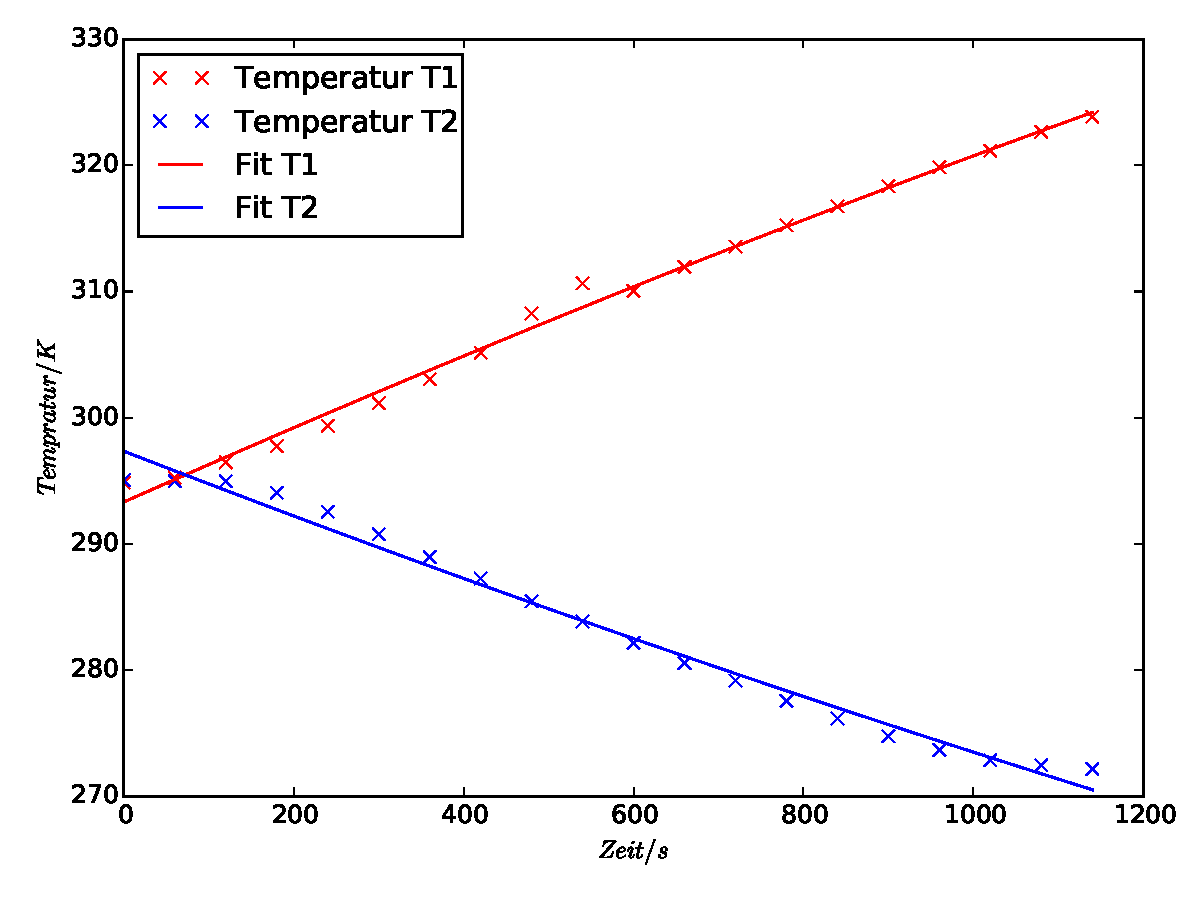
\includegraphics[width=0.78\textwidth]{Temperaturgraphik.pdf}
  \caption{Temperaturausgleichskurve.}
  \label{fig:temperaturgraphik}
\end{figure}
\newpage
\subsection{Temperaturausgleichskurve}
Die Näherung der Ausgleichskurven entstehen mit scientific Python und sind gegeben durch
\begin{equation}
  T(t)=At^2+Bt+C .
\end{equation}
Die Parameter für das erwärmte Reservoir $T_1$ sind
\begin{align*}
  A &=(-2\pm1)\cdot10^{-6}\si{\frac{\kelvin}{\second^2}}, \\
  B &=(3.0\pm0.2)\cdot10^{-2}\si{\frac{\kelvin}{\second}}, \\
  C &=(2.9331\pm0.0005)\cdot10^{2}\si{\kelvin}.
\end{align*}

Die Parameter für den anderen Behälter $T_2$ sind
\begin{align*}
  A &= (2\pm2)\cdot10^{-6}\si{\frac{\kelvin}{\second^2}}, \\
  B &= (-2.6\pm0.3)\cdot10^{-2}\si{\frac{\kelvin}{\second}}, \\
  C &= (2.9734\pm0.0006)\cdot10^{2}\si{\kelvin}.
\end{align*}

Die dazugehörigen Differentialquotienten für vier verschiedene Zeiten erhält man
durch die Gleichung
\begin{equation}
  \frac{dT}{dt}=2At+B
\end{equation}
und die Ergebnisse sind in nachfolgender Tabelle aufgeführt.

\begin{table}
  \centering
  \begin{tabular}{c c c}
    \toprule
    Zeit in s & $\frac{\symup{d}T_1}{\symup{d}t}/\frac{\si{\kelvin}}{\si{\second}}$
    & $\frac{\symup{d}T_2}{\symup{d}t}/\frac{\si{\kelvin}}{\si{\second}}$ \\
    \midrule
    300  &  0.028\pm0.002  & -0.025\pm0.003  \\
    600  &  0.027\pm0.003  & -0.023\pm0.004  \\
    900  &  0.025\pm0.004  & -0.022\pm0.005  \\
   1140  &  0.024\pm0.004  & -0.021\pm0.006  \\
   \bottomrule
 \end{tabular}
 \caption{Differentialquotienten.}
 \label{tab:Diffquo}
\end{table}


\subsection{Güteziffer}
Als nächstes soll die Güteziffer bestimmt werden. Dafür nutzt man die Gleichung
\eqref{eqn:gueteziffer_ideal} für die ideale Güteziffer und die Gleichung
\eqref{eqn:berechnung_gueteziffer} für die reale Güteziffer.
Die relative Abweichung von $v_\symup{real}$ zu $v_\symup{ideal}$ wird durch
\begin{equation}
  \Delta v_\symup{real} = \frac{v_\symup{real} - v_\symup{ideal}}{x_\symup{ideal}}
\end{equation}
berechnet. Das Ergebnis ist in untenstehender Tabelle zu sehen.
\begin{table}
  \centering
  \begin{tabular}{c c c c}
    \toprule
    Zeit in s & $v_\symup{ideal}$ &  $v_\symup{real}$ & relative Abweichung in \% \\
    \midrule
      300  &  28.96\pm0.39  &  1.87\pm0.15  & 93.5 \\
      600  &  11.11\pm0.05  &  1.69\pm0.18  & 84.8 \\
      900  &   7.30\pm0.02  &  1.60\pm0.23  & 78.1 \\
     1140  &   6.26\pm0.02  &  1.52\pm0.27  & 75.7 \\
   \bottomrule
 \end{tabular}
 \caption{Güteziffer und relative Abweichung.}
 \label{tab:Gütez}
\end{table}


\subsection{Massendurchsatz}
Für den Massendurchsatz wird die Verdampfungswärme $L=(1.998\pm0.007)\cdot10^{4}
\si{\frac{\joule}{\mol}}$ benötigt. Diese errechnet sich als
$L= -m \cdot R$ aus der Steigung einer Approximationgeraden mit $m=-2403\pm9$
der Wertepaare (p,T) der Dampfdruckkurve, multipliziert mit der universellen
Gaskonstante $R=8.314460\pm0.000005$.
\begin{figure}
  \centering
  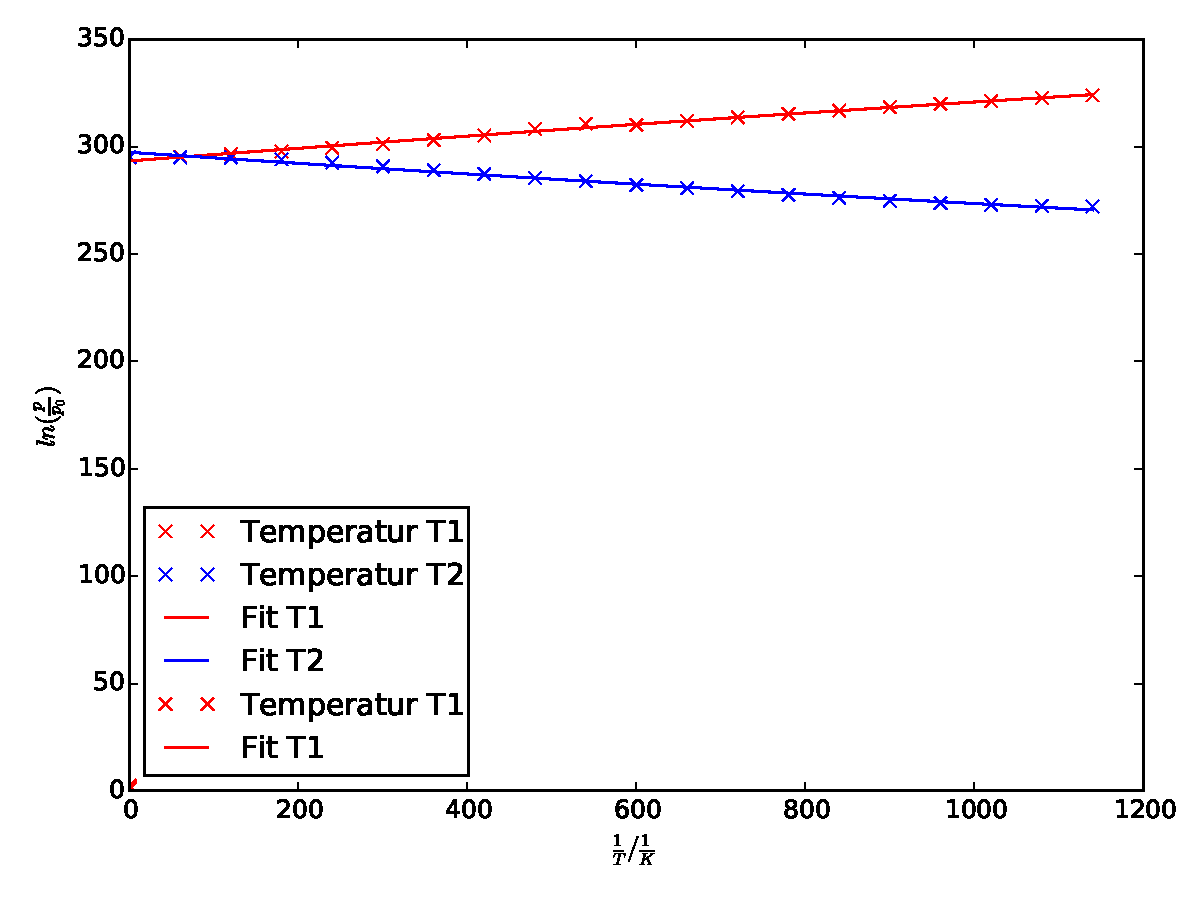
\includegraphics[width=0.9\textwidth]{prog/daten/Dampfdruckkurve.pdf}
  \caption{Verdampfungswärme.}
\end{figure}

Wenn die Werte in Gleichung \eqref{eqn:massendurchsatz} einsetzt werden, ergibt sich der Massendurchsatz.

\begin{table}
  \centering
\begin{tabular}{c c c c}
  \toprule
  Zeit in s & $\frac{\symup{d}Q_2}{\symup{d}t} \text{ in }\si{\joule}$
  & $\frac{\symup{d}m}{\symup{d}t}\text{ in }\si{\frac{\mol}{\second}}$
   & $\frac{\symup{d}m}{\symup{d}t} \text{ in }\si{\frac{\gram}{\second}}$\\
  \midrule
  300  &  -326.43\pm38.20  & 0.016\pm0.002  &  2.0\pm0.2  \\
  600  &  -308.55\pm48.55  & 0.015\pm0.002  &  1.9\pm0.3  \\
  900  &  -290.68\pm62.08  & 0.015\pm0.003  &  1.8\pm0.3  \\
 1140  &  -276.38\pm74.04  & 0.014\pm0.004  &  1.7\pm0.4  \\
 \bottomrule
\end{tabular}
\caption{Massendurchsatz.}
\label{tab:Massend}
\end{table}

\newpage
\subsection{Mechanische Kompressorleistung}
Die Dichte $\rho$, die für die Berechnung mechanischen Kompressorleistung
benötigt wird, kann berechnet werden, indem man die Gleichung der idealen Gase
umstellt
\begin{equation}
  pV=nRT \leftrightarrow \frac{pV}{T}=nR.
\end{equation}
Damit ergibt sich, da die Stoffmenge $n$ konstant bleibt,
\begin{equation}
  n_1=n_2
  \frac{p_0 V_0}{T_0}=\frac{p_2 V_2}{T_2}
\end{equation}
Da $ \rho V=m$ \leftrightarrow $V= \frac{m}{\rho}$ gilt, lässt sich $\rho$ mit
$\rho_2=\rho$ und $p_2=p_a$ wie folgt bestimmen
\begin{equation}
  \rho=\frac{\rho_0 T_0 p_a}{T_2 p_0}.
\end{equation}
Und mit Gleichung \eqref{eqn:kompressorleistung} ergibt sich für die mechanische
Kompressorleistung
\begin{equation}
N_\symup{mech}=\frac{1}{\kappa-1}\left(p_\symup{b} \sqrt[\kappa]
{\frac{p_\symup{a}}{p_\symup{b}}}-p_\symup{a}\right)
\frac{T_2 p_0}{\rho_0 T_0 p_\symup{a}} \frac{\symup{d}m}{\symup{d}t}.
\end{equation}

\begin{table}
  \centering
\begin{tabular}{c c c}
  \toprule
  Zeit in s & Dichte $\rho \text{ in }\frac{\si{\kilo\gram}}{\si{\meter}^3}$
  & Leistung $N_\symup{mech} \text{ in } \si{\watt}$   \\
  \midrule
  300  &  16.0\pm0.5   &  35\pm4  \\
  600  &  16.5\pm0.5   &  40\pm6  \\
  900  &  17.5\pm0.5   &  40\pm9  \\
 1140  &  17.7\pm0.6   &  42\pm11  \\
 \bottomrule
\end{tabular}
\caption{Massendurchsatz.}
\label{tab:Massend}
\end{table}
